\chapter{Experiments} \label{experiments_chapter}

In previous chapters I have presented the dataset (chapter \ref{chapter:data}), and discussed challenges which arise from its properties (chapter \ref{chapPreproc}). Next I described the neural network architectures (chapter \ref{neural_nets_chapter}) which served as building blocks for the models introduced in chapter \ref{model_chapter}. Now I want to connect all the parts together, elaborate on the trainining of the models (e.g. used optimizer, calculated metrics, hyperparameter choice) and analyze their results.

Let me recap the main challenges we face, and hypothesize about the ideal generation system. Firstly, the target summaries are really long. The ideal system should remember what has already been generated and shouldn't produce duplications. Secondly, the targets contain a lot of facts based on the input structured data. The ideal system should copy these facts from the input and reduce \emph{hallucinations}. Lastly, the generated text should be as close to English as possible \emph{while meeting the requirements described previously}.

\section{Development Methods}

The proposed models solve the task in \emph{end-to-end} manner. Given an input table $\boldsymbol{x}$ and the corresponding gold output summary $\boldsymbol{y}$ the model approximates the conditional probability of the latter conditioned on the former $p(\boldsymbol{y} | \boldsymbol{x})$. Following the maximum likelihood principle (e.g. section 5.5 in \citep{Goodfellow-et-al-2016}) the models are trained to minimize the cross-entropy loss (negative log likelihood) on the training set $\mathcal{D}$.(equation \ref{equation:negative_log_likelihood}).

\begin{equation} \label{equation:negative_log_likelihood}
    - \sum_{(\boldsymbol{x}, \boldsymbol{y}) \in \mathcal{D}}{log\ p_{model}(\boldsymbol{y} | \boldsymbol{x})}
\end{equation}

As explained in section \ref{subsection:high_level_encoder_decoder} the training happens under \emph{teacher-forcing} setting. The minimization is provided by stochastic gradient descent, specifically we opted to use one of the standard algorithms, Adam \citep{kingma2014adam}. Since this algorithm associates specific learning rate to each of the trainable network parameters, we modify only the initial learning rate parameter\footnote{It means that we don't try e.g. learning rate decay.}.

We report the loss value as well as the accuracy\footnote{the frequency with which the most probable token in the distribution generated by the model matches the gold token} of the model on the training set, to be able to detect \emph{underfitting} (this happens when a model is unable to achieve sufficiently low loss value on the training part of the dataset).

The main challenge is to obtain good results on previously unseen data. Therefore we report the loss value, and the accuracy of the model on the validation part of the dataset (also collected under \emph{teacher-forcing} setting). We consider the model with the lowest loss value and accuracy on the validation set to be the best.

\section{Generation} \label{section:generation}

As explained in section \ref{subsection:high_level_encoder_decoder}, during inference we want to find a sequence of tokens $y_1,\dots,y_n$ which maximizes the probability
\begin{equation}
    p_{model}(\boldsymbol{y} | \boldsymbol{x}) = \prod_{t=1}^N{p_{model}(y_t|y_1,\dots,y_{t-1}, \boldsymbol{x})}
\end{equation}

Since it is computationally  unfeasible to compute the probabilities of all the output sequences and to choose the best one we only approximate the optimal sequence.

\subsection{Greedy Decoding}

Greedy Decoding provides the simplest approximation of the optimal sequence. At each time-step we take the most probable token under the model distribution as the output. The process ends when the \emph{\textless EOS\textgreater} token is generated.
\begin{align*}
    \hat{y}_1 &= \argmax_{y'}{p_{model}(y' | \boldsymbol{x})} \\
    \hat{y}_2 &= \argmax_{y'}{p_{model}(y' | \hat{y}_1, \boldsymbol{x})} \\
    &\dots \\
    <EOS> &= \argmax_{y'}{p_{model}(y' | \hat{y}_1,\dots,\hat{y}_{n'}, \boldsymbol{x})}
\end{align*}

The suboptimality of the algorithm can be seen on a simple example. E.g. let's say that we have a training corpus consisting of sentences describing my eating habits. The corpus consists of sentences "I eat a banana", "I eat a peach", "I eat a goulash" and two repetitions of sentence "I eat an apple". Starting from the state after generating subsequence "I eat", the greedy decoder would pick ``a'' as the most probable continuation of the sequence. However the optimal solution would have picked "an", because none of the possible continuations of subsequence "I eat a" is as probable as "I eat an apple" which is the most occuring sentence in the corpus.

\subsection{Beam Search Decoding}

Beam Search builds on the greedy decoding approach. We keep track of $k$ most promising \emph{hypotheses} (and associated hidden states). A hypothesis is a sequence of generated tokens $y_1,\dots,y_{n'}$. We compute its score (equation \ref{equation:hypothesis_score}).
\begin{equation} \label{equation:hypothesis_score}
    score(y_1,\dots,y_{n'}) = \sum_{i=1}^{n'}{\log{p(y_i | y_1, \dots, y_{i-1}, \boldsymbol{x})}}
\end{equation}

At each time-step we expand all the hypotheses (take $k$ most probable tokens under the respective hypothesis, which will result in $k^2$ possibilities), and choose $k$ with the highest score. $k$ is called the \emph{beam size}. An example of the approach can be seen in figure \ref{figure:beam_search}. There exist several options what to do when some hypothesis expands to \emph{\textless EOS \textgreater} token. The finished hypothesis can be put aside and the generation continues until $T$-th time-step ($T$ is another hyperparameter of the algorithm), or until at least $N$ hypotheses are finished. I choose yet another option, to end the generation right after the first \emph{\textless EOS\textgreater} is generated.

\begin{figure}[!h]
    \centering
    \includegraphics[scale=0.2]{img/beam_search.png}
    \caption{\centering Beam-Search decoding, excerpt from the slides to lecture about Machine Translation, Seq2Seq and Attention on Stanford \url{http://web.stanford.edu/class/cs224n/}} \label{figure:beam_search}
\end{figure}

\subsection{Postprocessing}

The models are trained to generate lowercased Byte Pair Encoded sequences. During the postprocessing I merge the tokens belonging to one word together (e.g. \emph{"contribu$\star$ tor"} $\rightarrow$ \emph{"contributor"}), split the tokens of named entities (e.g. \emph{"LeBron\_James"} $\rightarrow$ \emph{"LeBron James"}) and uppercase the first letter of a sentence.

\section{Regularization}

Two regularization methods are used, Dropout and Scheduled Sampling \citep{bengio2015scheduled}.

"The key idea of Dropout is to randomly drop units (along with their connections) from the neural network during training." \citep{srivastavaDropout2014}. A unit is dropped with probability $p$ that can be set as a hyperparameter. (e.g. $p = 0$ would mean no dropout)  We apply the dropout on the outputs of the LSTM cells.

The Scheduled Sampling aims to minimize the difference between training and inference. \citep{bengio2015scheduled} note that using any of the two generation techniques described above (section \ref{section:generation}) the model can get to the "state space that is very different from those visited from the  training distribution and for which it doesn’t know what to do". They propose to "bridge the gap" by feeding either gold $y_{t-1}$ or the prediction of the model $\hat{y}_{t-1}$ as the input at $t$-th time-step. The decision whether to use gold is made independently for each input with probability $p'$ which is another hyperparameter of the training. They propose to decay $p'$ over time with similar strategies as used with learning rate.

\section{Evaluation Methods}

During evaluation I want to measure which model resembles the hypothetical ideal model the most. To do so, I report the BLEU score \citep{papineni2002} of the postprocessed generated summaries on the validation and test sets. Although it is the gold standard, there are many people arguing against its usage as a performance metric \citep{celikyilmaz2021evaluation}, and I found that the networks producing more factually correct statements doesn't score better. Therefore I also manually evaluate a subset of the generated summaries.

\subsection{Manual Evaluation}

I used a pseudo random generator to pick 8 different data points, 4 from the validation and 4 from test set\footnote{Specifically samples $132$, $319$, $475$ and $709$ from the validation set and samples $16$, $247$, $585$ and $671$ from the test set}. I looked at the factual correctness (how many of the generated numbers describing team and player statistics are based on the input tabular data), and factual recall (how many of the entities mentioned in the gold summaries are present in the generated ones). Due to time-requirements of the process, only the best model\footnote{In the respective sections I explain why I think the selected model is the best one.} is manually evaluated. Therefore manual evaluation should show the differences between approaches and architectures rather than between variations of the same model.

\subsection{Ommited Evaluation Methods}

\citep{wiseman2017} proposed three custom automated metrics to evaluate the performance of their models. They call them \emph{Content Selection} ("how well the generated document matches the gold document in terms of selecting which records to generate"), \emph{Relation Generation} ("how well the system is able to generate text containing factual (i.e., correct) records") and \emph{Content Ordering} ("how well the system orders the records it chooses to discuss"). The metrics are implemented in outdated neural network framework \emph{Torch} and I wasn't able to execute it on my computers. After discussions with my advisor we agreed to not adopt these methods.

\section{Baseline Model}

At first I would like to summarize my expectations. \citep{wiseman2017} note that even models with explicit copy mechanisms tend to \emph{hallucinate} the facts. However they do not show the results of any baseline without copying. We expect the baseline to generate a fairly good English, even though the summaries should not be factually correct.

I searched through the hyperparameter space (possible combinations of learning rates, dropout probability $p$, hidden state dimensionality etc.) until the generated language as well as the numerical results haven't fulfilled the expectations at least by half.

The overall architecture of the baseline model is discussed in section \ref{section:baseline_model}. Figure \ref{figure:hyperparameters_baseline} shows the hyperparameter choice for discussed baseline models.

\begin{figure}[h]
    \scalebox{0.8}{
    \begin{tikzpicture}
    \node(embeddings) [] {
        \small
        \begin{tabular}{ll}
            \toprule
            {} & \textbf{Embedding} \\
            \pulrad{\textbf{Token}} & \textbf{Dimensionality} \\
            \midrule
            \textbf{$record.type$} & 300 \\
            \textbf{$record.home\_away$} & 300 \\
            \textbf{$record.value$} & 600 \\
            \textbf{$record.entity$} & 600 \\
            \textbf{$summary\ token$} & 600
        \end{tabular}
    };
    \node(hidden) [above left=-20.7mm and 5mm of embeddings] {
        \small
        \begin{tabular}{ccc}
            \toprule
            \textbf{Hidden States} & {} & {} \\
            \textbf{Dimensionality} & \pulrad{\textbf{Learning Rate}} & \pulrad{\textbf{Batch Size}} \\
            \midrule
            600 & 0.001 & 16
        \end{tabular}
    };
    \end{tikzpicture}
    }
    \caption{Hyperparameter settings for baseline models.} \label{figure:hyperparameters_baseline}
\end{figure}

The first baseline model is trained without any regularization, the second one with dropout on the output LSTM units with $p_{dropout} = 0.3$ (the probability that the unit is dropped is $0.3$) and scheduled sampling with constant rate of $0.8$ (the probability that the gold output from the previous timestep is used as the actual input is $0.8$).

\subsection{Results}

Baseline model wasn't able to capture the relationships between the input tabular data and the output summaries (the best configuration achieved perplexity $10.59$). We found that dropout helps to reduce overfitting while scheduled sampling improved the quality of the generated summaries. (We present only models which achieved reasonable performance.) The quality of generated summaries is further improved with beam search. Although the statement contradicts the calculated BLEU scores (as the score decreased after introducing beam search), the summaries contain more natural language and less repetitions. The expectations are fulfilled in terms of \emph{hallucinations}, as the model makes up \emph{almost all the factual statements}.

\begin{table}[h]
    \centering
    \scalebox{0.8}{
    \begin{tabular}{lccccc}
        \toprule
        {} & \textbf{Validation} & \textbf{Validation} & \textbf{Test} & \textbf{Entity} & \textbf{Correct} \\
        \pulrad{\textbf{Model}} & \textbf{Perplexity} & \textbf{BLEU} & \textbf{BLEU} & \textbf{Recall} & \textbf{Facts} \\
        \midrule
        BN$_G$ & {} & 9.04 & 9.10 & -- & -- \\
        BN$_{B5}$ & \pulrad{12.68} & 8.73 & 8.55 & -- & -- \\
        \hline
        BR$_G$ & {} & 10.0 & 10.47 & -- & -- \\
        BR$_{B5}$ & \pulrad{10.59} & 9.99 & 10.6 & 37.35\% & 8.03\% \\
        \bottomrule
        \multicolumn{4}{l}{\footnotesize{$_{G}$ - Greedy Decoding}} \\
        \multicolumn{4}{l}{\footnotesize{$_{B5}$ - Beam search decoding, beam size $=5$}} \\
        \multicolumn{4}{l}{\footnotesize{BN - Baseline, non-regularized}} \\
        \multicolumn{4}{l}{\footnotesize{BR - Baseline, regularized (dropout $0.3$, scheduled sampling $0.8$)}}
    \end{tabular}
    }
    \caption{Performance metrics on the baseline models.} \label{table:metrics_baseline}
\end{table}

Figure \ref{figure:baseline_generated} shows an example generated by the regularized baseline model with beam search decoding. We observe\footnote{We opted to not show the same tabular information multiple times. A part of the table corresponding to the generated summary can be found in figure \ref{figure:samplesummary}} that the score, the winning-loosing records\footnote{\emph{"The Raptors ( 21 - 15)"} means that Raptors have won $21$ matches and lost $15$ matches this season.} as well as all the individual statistics are \emph{hallucinated}. We found that the model repeatedly (over multiple observed summaries) mentions the same players and uses the same numbers. This experiment thus supports our assumptions. Statistics in table \ref{table:metrics_baseline} show that only about $8$ \% of the numbers aren't \emph{hallucinated} and that the recall is lower than $35$ \%. Therefore we can conclude that model learned to produce probable numbers and names of star players of the respective teams. 


\begin{figure}[h]
    \scalebox{0.85}{
    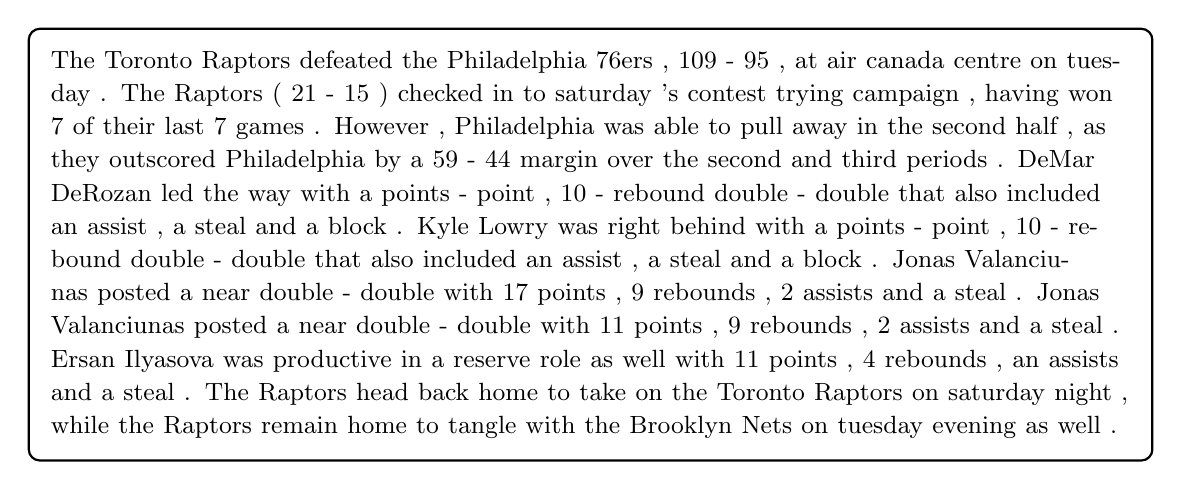
\begin{tikzpicture}
    \node(summary) [rectangle, draw,thick,fill=blue!0,text width=39em, rounded corners, inner sep =8pt, minimum height=1em]{
        \baselineskip=100pt
        \small
        The Toronto Raptors defeated the Philadelphia 76ers , 109 - 95 , at air canada centre on tuesday . The Raptors ( 21 - 15 ) checked in to saturday 's contest trying campaign , having won 7 of their last 7 games . However , Philadelphia was able to pull away in the second half , as they outscored Philadelphia by a 59 - 44 margin over the second and third periods . DeMar DeRozan led the way with a points - point , 10 - rebound double - double that also included an assist , a steal and a block . Kyle Lowry was right behind with a points - point , 10 - rebound double - double that also included an assist , a steal and a block . Jonas Valanciunas posted a near double - double with 17 points , 9 rebounds , 2 assists and a steal . Jonas Valanciunas posted a near double - double with 11 points , 9 rebounds , 2 assists and a steal . Ersan Ilyasova was productive in a reserve role as well with 11 points , 4 rebounds , an assists and a steal . The Raptors head back home to take on the Toronto Raptors on saturday night , while the Raptors remain home to tangle with the Brooklyn Nets on tuesday evening as well .
    };
    \end{tikzpicture} }
    \caption{\centering A summary generated by the baseline model. The corresponding gold summary and input table is shown in figure \ref{figure:samplesummary}.} \label{figure:baseline_generated}
\end{figure}

\section{Joint-Copy Model}

The Joint-Copy Model is expected to produce more factually correct statements. \citep{wiseman2017} select this model as their baseline. Due to massive preprocessing that we introduced, the results we obtained aren't comparable to theirs. (E.g. Wiseman et al. report BLEU $10.41$ while we obtained similar scores with \emph{simpler baseline model}.)

The additional complexity of the model increases the memory demands. The\-refore we use lower dimensional embeddings, hidden states and smaller batch size as presented in figure \ref{figure:hyperparameters_copy_low_lr} to be able to train on the GPUs on the AIC. Compared to the baseline model we obtained the best results when training with $5$-times lower learning rate. Regularization methods didn't provide any significant advantage over the unregularized case.

\begin{figure}[h]
    \scalebox{0.8}{
    \begin{tikzpicture}
    \node(embeddings) [] {
        \small
        \begin{tabular}{ll}
            \toprule
            {} & \textbf{Embedding} \\
            \pulrad{\textbf{Token}} & \textbf{Dimensionality} \\
            \midrule
            \textbf{$record.type$} & 300 \\
            \textbf{$record.home\_away$} & 300 \\
            \textbf{$record.value$} & 500 \\
            \textbf{$record.entity$} & 500 \\
            \textbf{$summary\ token$} & 500
        \end{tabular}
    };
    \node(hidden) [above left=-20.7mm and 5mm of embeddings] {
        \small
        \begin{tabular}{ccc}
            \toprule
            \textbf{Hidden States} & {} & {} \\
            \textbf{Dimensionality} & \pulrad{\textbf{Learning Rate}} & \pulrad{\textbf{Batch Size}} \\
            \midrule
            500 & 0.0002 & 8
        \end{tabular}
    };
    \end{tikzpicture}
    }
    \caption{Hyperparameter settings for joint-copy models.} \label{figure:hyperparameters_copy_low_lr}
\end{figure}

\subsection{Results}

We see the first major improvement in the BLEU score (more than 2 points) as well as in the manually evaluated metrics (almost $6$-times better factual correctness). However the model fails in recognition of the structure of the table.

While it is able to copy facts, many times it copies statistics of wrong players (e.g. it learns that most of the time $5$-th player from the input records is most important, therefore it mentions the $5$-th player even if he scored unremarkable amount of points).

We also spotted that model learned that it is more probable that home team wins. Therefore it produces sentence similar to \emph{"The Denver Nuggets ( 11 - 17 ) defeated the Los Angeles Lakers ( 5 - 23 ) 111 - 107 on friday at the pepsi center in Denver . "} even if the score was reversed (\emph{107 - 111} in favour of the Lakers).

Also the model relatively often generates a sequence of tokens which cannot be seen in the training data which causes \emph{cycling} (model generates one sentence multiple times), which results in exceeding the maximal allowed length of a summary (We don't allow the model to generate longer sequence than the longest one seen in the dataset (849 tokens)). The phenomenon can be seen in figure \ref{figure:copy_low_lr_generated}.

Contrary to observations on the baseline model neither greedy decoding nor beam search managed to significantly outperform the other method.

\begin{table}[h]
    \centering
    \scalebox{0.8}{
    \begin{tabular}{lccccc}
        \toprule
        {} & \textbf{Validation} & \textbf{Validation} & \textbf{Test} & \textbf{Entity} & \textbf{Correct} \\
        \pulrad{\textbf{Model}} & \textbf{Perplexity} & \textbf{BLEU} & \textbf{BLEU} & \textbf{Recall} & \textbf{Facts} \\
        \midrule
        Copy$_G$ & {} & 12.48 & 12.6 & 37.35\% & 47.29\% \\
        Copy$_{B5}$ & \pulrad{9.87} & 12.19 & 12.5 & 39.76\% & 47.13\% \\
        \bottomrule
        \multicolumn{4}{l}{\footnotesize{$_{G}$ - Greedy Decoding}} \\
        \multicolumn{4}{l}{\footnotesize{$_{B5}$ - Beam search decoding, beam size $=5$}} \\
    \end{tabular}
    }
    \caption{Performance metrics on the joint-copy models.} \label{table:metrics_copy_low_lr}
\end{table}

\begin{figure}[h]
    \scalebox{0.85}{
    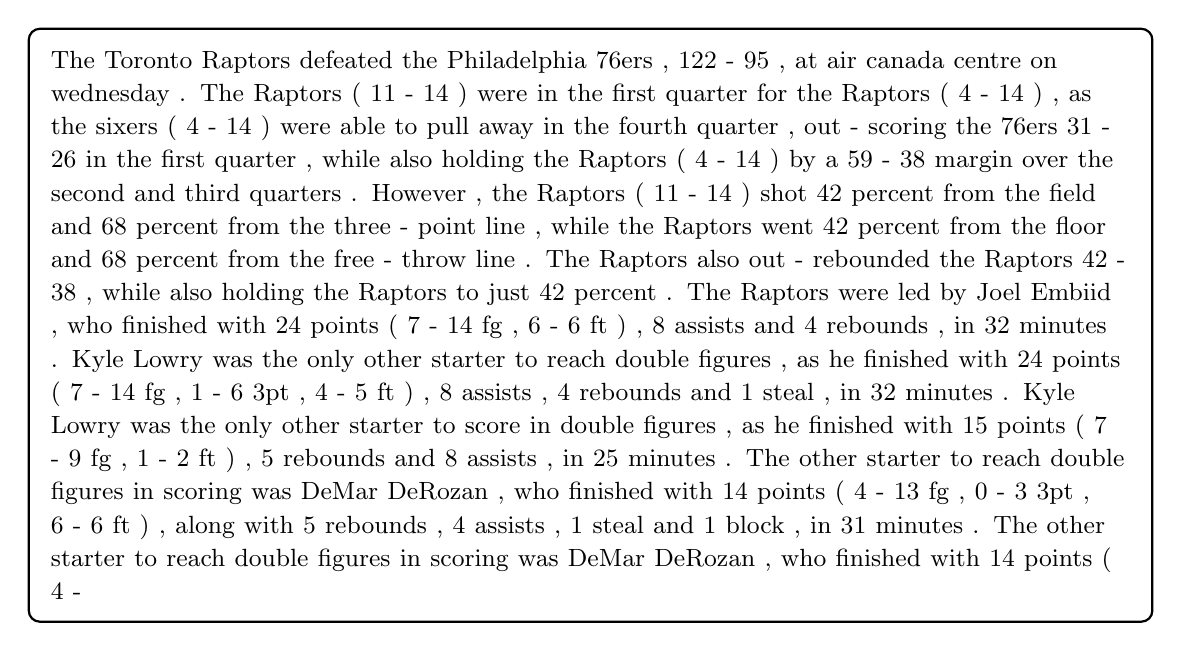
\begin{tikzpicture}
    \node(summary) [rectangle, draw,thick,fill=blue!0,text width=39em, rounded corners, inner sep =8pt, minimum height=1em]{
        \baselineskip=100pt
        \small
        The Toronto Raptors defeated the Philadelphia 76ers , 122 - 95 , at air canada centre on wednesday . The Raptors ( 11 - 14 ) were in the first quarter for the Raptors ( 4 - 14 ) , as the sixers ( 4 - 14 ) were able to pull away in the fourth quarter , out - scoring the 76ers 31 - 26 in the first quarter , while also holding the Raptors ( 4 - 14 ) by a 59 - 38 margin over the second and third quarters . However , the Raptors ( 11 - 14 ) shot 42 percent from the field and 68 percent from the three - point line , while the Raptors went 42 percent from the floor and 68 percent from the free - throw line . The Raptors also out - rebounded the Raptors 42 - 38 , while also holding the Raptors to just 42 percent . The Raptors were led by Joel Embiid , who finished with 24 points ( 7 - 14 fg , 6 - 6 ft ) , 8 assists and 4 rebounds , in 32 minutes . Kyle Lowry was the only other starter to reach double figures , as he finished with 24 points ( 7 - 14 fg , 1 - 6 3pt , 4 - 5 ft ) , 8 assists , 4 rebounds and 1 steal , in 32 minutes . Kyle Lowry was the only other starter to score in double figures , as he finished with 15 points ( 7 - 9 fg , 1 - 2 ft ) , 5 rebounds and 8 assists , in 25 minutes . The other starter to reach double figures in scoring was DeMar DeRozan , who finished with 14 points ( 4 - 13 fg , 0 - 3 3pt , 6 - 6 ft ) , along with 5 rebounds , 4 assists , 1 steal and 1 block , in 31 minutes . The other starter to reach double figures in scoring was DeMar DeRozan , who finished with 14 points ( 4 -
    };
    \end{tikzpicture} }
    \caption{\centering A summary generated by the joint-copy model. The corresponding gold summary and input table is shown in figure \ref{figure:samplesummary}.} \label{figure:copy_low_lr_generated}
\end{figure}

\section{Content Selection Encoder with Joint-Copy Decoder}

\citep{puduppully2019datatotext} introduced two new concepts. The first one, the Content Selection (CS) (discussed in section \ref{subsection:content_selection}) uses self-attention to incorporate \emph{context awareness}. Basically it should mean that the encoded record representation should be aware about the most important records related to itself. \citep{puduppully2019datatotext} report that CS alone contributes to the quality of the generated summaries. We expect the model with CS to resolve the problem of mixing statistical information of multiple players.

The hyperparameter configuration rests the same as in Joint-Copy model (figure \ref{figure:hyperparameters_copy_low_lr}).

\subsection{Results}

The summaries produced by the model are richer in structure, as they mention more entities from the input tables ($44.58$ \% vs $39.76$ \% for the Copy model). However we observe that many times model doesn't copy the players name (it only learns to copy numbers). E.g. it generates a sentence \emph{"The Raptors were led by DeMar DeRozan , who finished with a team - high of 26 points ( 9 - 16 fg , 0 - 2 3pt , 8 - 9 ft ) , to go along with 7 rebounds and 5 assists ."} where there would be $8 / 9$ numbers correct if the name wasn't \emph{DeMar DeRozan} but \emph{Marc Gasol}. This causes the model to score less on the factual correctness metric ($42.22$ \% vs $47.13$ \% for the Copy Model). Regarding BLEU score we see an improvement of about $1$ point.

\begin{table}[h]
    \centering
    \scalebox{0.8}{
    \begin{tabular}{lccccc}
        \toprule
        {} & \textbf{Validation} & \textbf{Validation} & \textbf{Test} & \textbf{Entity} & \textbf{Correct} \\
        \pulrad{\textbf{Model}} & \textbf{Perplexity} & \textbf{BLEU} & \textbf{BLEU} & \textbf{Recall} & \textbf{Facts} \\
        \midrule
        CopyCS$_G$ & {} & 13.53 & 13.62 & -- & -- \\
        CopyCS$_{B5}$ & \pulrad{9.93} & 13.96 & 13.54 & 44.58\% & 42.22\% \\
        \bottomrule
        \multicolumn{4}{l}{\footnotesize{CopyCS - Joint-Copy decoder $+$ Content Selection encoder}} \\
        \multicolumn{4}{l}{\footnotesize{$_{G}$ - Greedy Decoding}} \\
        \multicolumn{4}{l}{\footnotesize{$_{B5}$ - Beam search decoding, beam size $=5$}} \\
    \end{tabular}
    }
    \caption{Performance metrics on the joint-copy model with content selection encoder.} \label{table:metrics_copy_content_selection}
\end{table}

I would like to note that I don't think I came even close to the apex of the performance of this configuration as many summaries still show indications of underfitting (e.g. sequences like \emph{"TEAM-A defeated TEAM-A"}). Therefore I do not show an example of the summary generated by the model (as it contains sentences of the same quality as the ones generated by the joint-copy model).

\section{Content Selection and Planning}

The second concept introduced by \citep{puduppully2019datatotext} is the Content Planning Decoder (discussed in section \ref{subsection:content_planning}). The generation is divided into two parts. In the first one, we generate a sequence of pointers to the input records which contain the most essential information from the table. In the second phase we generate the summary according to records pointed to by the extracted pointers. Multitude of added architectures (content selection attention, content planning attention, content planning LSTM) increased even more the memory demands. Therefore we again reduced the embedding and hidden state dimensionalities (figure \ref{figure:hyperparameters_content_selection_and_planning}).

\begin{figure}[h]
    \scalebox{0.8}{
    \begin{tikzpicture}
    \node(embeddings) [] {
        \small
        \begin{tabular}{ll}
            \toprule
            {} & \textbf{Embedding} \\
            \pulrad{\textbf{Token}} & \textbf{Dimensionality} \\
            \midrule
            \textbf{$record.type$} & 300 \\
            \textbf{$record.home\_away$} & 300 \\
            \textbf{$record.value$} & 450 \\
            \textbf{$record.entity$} & 450 \\
            \textbf{$summary\ token$} & 450
        \end{tabular}
    };
    \node(hidden) [above left=-20.7mm and 5mm of embeddings] {
        \small
        \begin{tabular}{ccc}
            \toprule
            \textbf{Hidden States} & {} & {} \\
            \textbf{Dimensionality} & \pulrad{\textbf{Learning Rate}} & \pulrad{\textbf{Batch Size}} \\
            \midrule
            500 & 0.0002 & 8
        \end{tabular}
    };
    \end{tikzpicture}
    }
    \caption{Hyperparameter settings for content selection and planning models.} \label{figure:hyperparameters_content_selection_and_planning}
\end{figure}

Content Planning reduces the size of the table, and \emph{arranges} the records into the same order in which they appear in the gold summary. There are two aspects of this solution which should help the model to generate better summaries. Firstly, the input sequences of records become less complex (the maximal length of content plan is $92$ compared to more than $800$ for the original tables). Secondly, the records are ordered in the same way as they should appear in the summary. \citep{puduppully2019datatotext} show that this approach led them to really promising results (e.g. they obtained BLEU score of about $16$).

\section{Results}

We weren't able to develop sufficiently good models. The content planning part of the model overfitted in the first epoch. Since we weren't able to set up training with two optimizers (because of some implementation issues with \emph{persistent tf.GradientTape}), we tried to regularize the content planning part more (e.g. to apply bigger dropout than on the text generation part), train the content planning less (by using a similar algorithm to scheduled sampling, when we decide with probability $p$ for each batch whether to train the content planning part or not), use even lower learning rates. The shortness of time was the biggest issue we faced. The training of one epoch (one pass through the dataset) takes about 5 hours. Therefore we have to wait for about 3 days to see if the model generalizes well on the test set or not.

The best model we managed to train was regularized using dropout rate $0.5$ on all the LSTM cells (in the content plan decoder, in text decoder). The generated summaries were of really low quality (e.g. one of generated sentences hallucinated a miraculous performance by Kemba Walker :  \emph{"Kemba Walker , who tallied 7 points , 7 assists , 1 rebound , 2 steals and 0 block , in 2 minutes"}). The performance metrics do not recognize how bad the model actually is, as it scored better than the Joint-Copy model (table \ref{table:metrics_csap}).

\begin{table}[h]
    \centering
    \scalebox{0.8}{
    \begin{tabular}{lccccc}
        \toprule
        {} & \textbf{Validation} & \textbf{Validation} & \textbf{Test} & \textbf{Entity} & \textbf{Correct} \\
        \pulrad{\textbf{Model}} & \textbf{Perplexity$_1$} & \textbf{BLEU} & \textbf{BLEU} & \textbf{Recall} & \textbf{Facts} \\
        \midrule
        CS\&P$_G$ & 9.93 & 13.07 & 13.08 & 44.58\% & -- \\
        \bottomrule
        \multicolumn{4}{l}{\footnotesize{CS\&P Content Selection and Planning model}} \\
        \multicolumn{4}{l}{\footnotesize{$_{G}$ - Greedy Decoding}} \\
        \multicolumn{4}{l}{\footnotesize{$_{B5}$ - Beam search decoding, beam size $=5$}} \\
        \multicolumn{4}{l}{\footnotesize{$_1$ - Validation Perplexity of text decoding from gold content plans}}
    \end{tabular}
    }
    \caption{Performance metrics on the joint-copy model with content selection encoder.} \label{table:metrics_csap}
\end{table}

\section{Ordered Tables}

Since we haven't managed to obtain sufficient results using any of the previously proposed methods we try to make the task easier. Going through the gold content plans as well as the ones generated by Content Selection and Planning model we spotted that their structure follows a simple pattern. At first the teams are presented, then there is some information about the best players and about players who performed surprisingly well.

Therefore we order the input records in a similar way. The first records in the ordered sequence belong to home and away teams. The remaining records contain information about all the players, who are ordered by their point-totals in the respective match. The size of the table remains the same 

\section{Shortened Tables}

There will be section with my best results with BLEU of $15.5$.

\section{Overall Comparison}

There will be section with notes to each implemented model, table with their performance metrics etc. etc.

\section{Implementation Details}

As stated in the introduction this thesis is highly theoretical and experimental. The implementation serves as proof-of-concept and doesn't aim to be used in the production.

All the models and preprocessing methods were developed in \emph{python 3.8} and \emph{tensorflow 2.4.1}. However the code is compatible with \emph{python 3.6} and \emph{tensorflow 2.3} (the versions used on Artifical Intelligence Cluster (AIC) where the training was executed). The implementation is divided into two modules, \emph{preprocessing} and \emph{training}.

\subsection{Preprocessing Module}

The preprocessing happens in four steps.
\begin{enumerate}
    \item Filtering out the faulty data-points (section \ref{cleaning_section}) from the original dataset.
    \item Extraction and transformation of the summaries from the cleaned dataset.
    \item Byte Pair Encoding of the summaries. (As explained in section \ref{bpeSection} I use the \emph{subword-nmt} module by \citep{sennrich2016}.)
    \item Construction of the dataset from the encoded summaries and the cleaned data. 
\end{enumerate}
Each step is implemented in \emph{python} and the steps are connected by a shell script.

\subsection{Training Module}

The training module contains implementation of layers and models discussed in previous chapters as well as training, evaluation and inference methods. It makes use of \emph{graph execution}\footnote{\url{https://www.tensorflow.org/guide/intro_to_graphs}} during training and \emph{eager execution}\footnote{\url{https://www.tensorflow.org/guide/eager}} during evaluation and prediction.

The code is available at \url{https://github.com/gortibaldik/TTTGen/}.